\documentclass{article}

\usepackage{graphicx}
\usepackage{subcaption}
\usepackage{amsmath}
\usepackage{float}
\usepackage{listings}
\usepackage{xcolor}
\usepackage{float}

\lstset{
    language=Java,
    basicstyle=\ttfamily\footnotesize,
    breaklines=true,
    numbers=left,
    stepnumber=1,
    numbersep=5pt,
    showspaces=false,
    showstringspaces=false,
    tabsize=2
}

\title{Sistemas Distribuídos - Atividade 1: Serialização}
\author{André Filipe de Medeiros - 542104}
\date{\today}

\begin{document}
\maketitle

\newpage
\section{Resumo}
A presente atividade visa avaliar o impacto de diferentes protocolos de serialização no tamanho de mensagens trocadas entre processos (cliente e servidor) em Java. Analizaram-se cinco tipos de serialização: padrão do Java (com e sem customização), JSON, XML e Protobuf, em dois cenários: um com baixo volume de dados (requisição de compra) e outro com maior volume (agenda de contatos). Com auxílio do Wireshark, comparou-se o número de bytes enviados em cada contexto. Evidenciou-se que a serialização pelo protocolo Protobuf foi a mais eficiente em termos de compactação.

\section{Discussão Técnica}

\subsection{Serialização}
A serialização é um procedimento responsável por transformar um objeto ou estrutura de dados em um formato possível de ser armazenado ou transmitido. Nesse sentido, a serialização é fundamental para que sistemas diferentes se comuniquem no contexto de computação distribuída.

Atualmente, existem diferentes protocolos que implementam a serialização como a serialização padrão do Java, serialização customizada do Java, JSON, XML e Protobuf. 

\section{Metodologia}

\subsection{Código}
Os códigos foram escritos na linguagem Java. Programou-se dois programas para cada protocolo e cenário. O primeiro programa é referente ao processo servidor, que foi executado no endereço \textit{localhost} e porta $6789$. O papel do processo servidor é de apenas receber a mensagem do processo cliente e imprimir a mensagem no terminal. Enquanto, no processo cliente, instanciam-se objetos e os enviam ao processo servidor. 

Ao todo, criaram-se códigos a dez cenários:
\begin{equation}
    N = 5 \;(prot.\, de \,serializacao) \times 2 \;(compra\, e\, agenda) = 10
\end{equation}
Os códigos estão disponíveis em: {https://github.com/andredemedeiros/serializations.git}

\subsection{Captura de pacotes}
A captura de pacotes ocorreu em três etapas. A primeira etapa foi referente a inicialização de captura de pacotes através do Wireshark. Na segunda etapa, executaram-se os processos servidor e cliente, respectivamente, para que os objetos fossem serializados e transmitidos. 
Por fim, os dados da captura foram salvos em formato \textit{.pcap} e estão disponíveis no repositório. 

\begin{figure}[H]
    \centering
    \caption{Captura de pacotes da serialização padrão no cenário de requisição de compra.}
    \begin{subfigure}[b]{0.7\textwidth}
        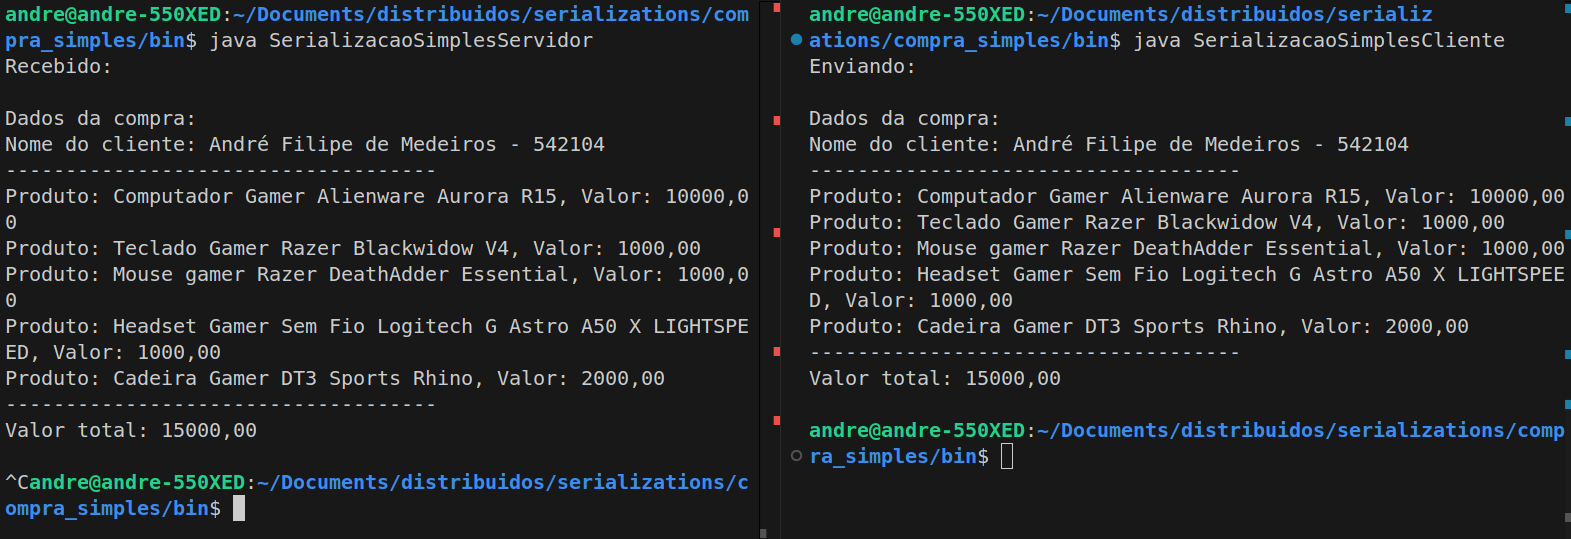
\includegraphics[width=\textwidth]{imgs/compra_simples_term.png}
        \caption{Execução dos processos servidor e cliente com protocolo de serialização padrão do Java.}
        \label{fig:clock_original}
    \end{subfigure}%

    \begin{subfigure}[b]{0.7\textwidth}
        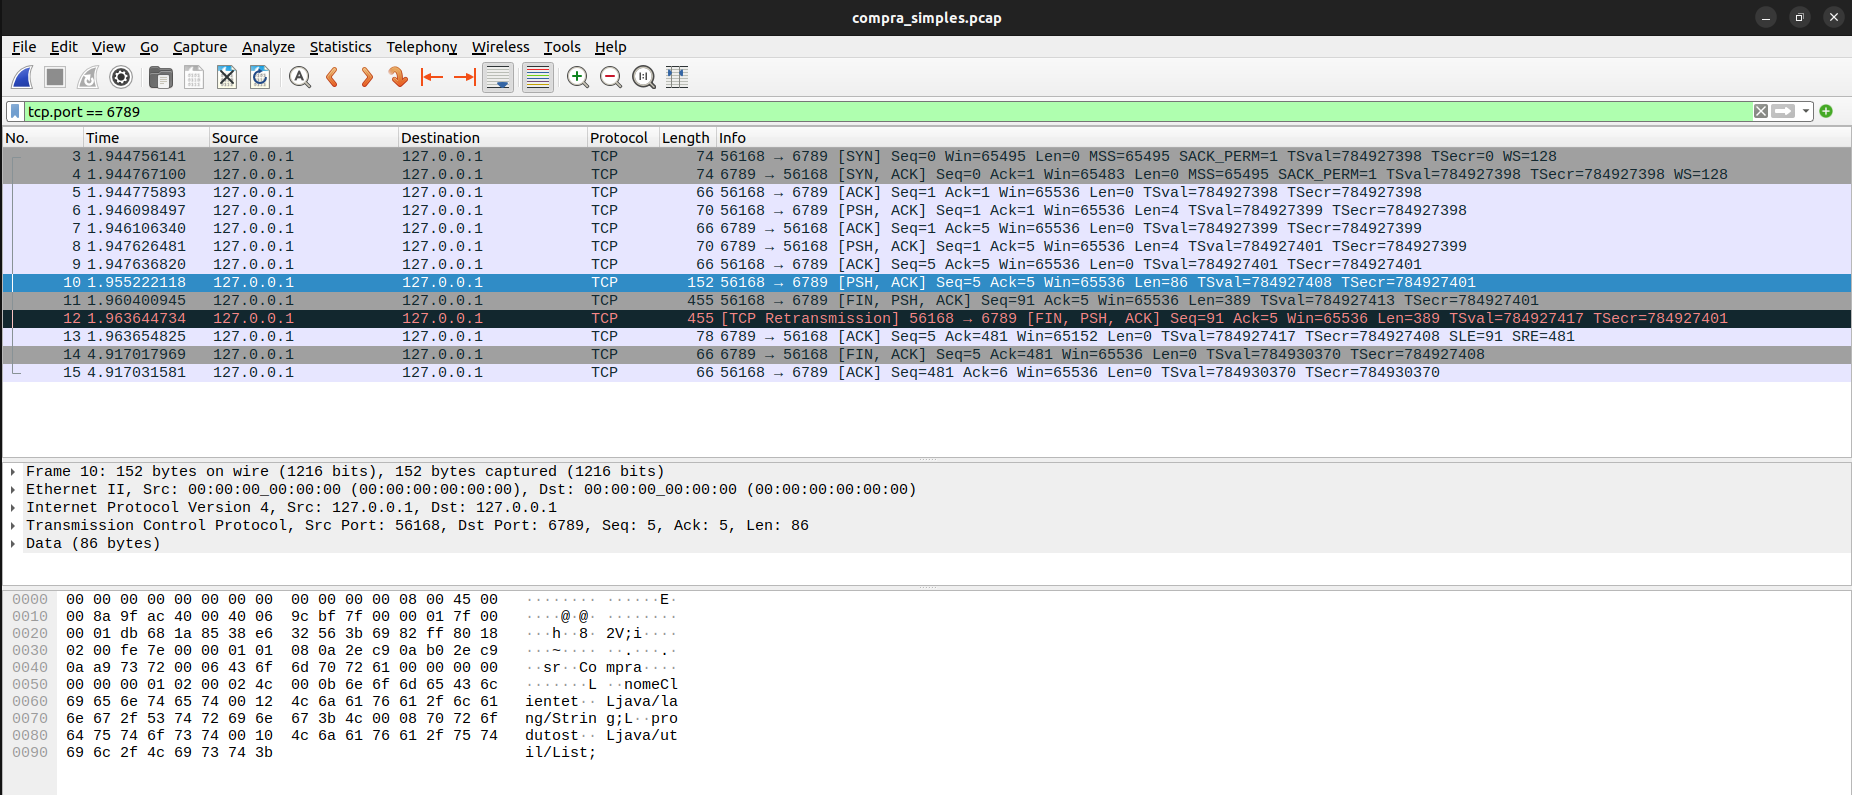
\includegraphics[width=\textwidth]{imgs/compra_simples_wire.png}
        \caption{Captura dos pacotes trocados pelos processos cliente e servidor com protocolo de serialização padrão do Java.}
        \label{fig:clock_300dpi}
    \end{subfigure}%
    \label{fig:clock_comparison}
\end{figure}

Aplicou-se o mesmo procedimento de captura de pacotes em todos cenários.

\subsection{Cálculo de tamanho de pacotes}
Os pacotes do cenário que simula uma requisição de compra, possui um volume considerávelmente menor em comparação com os
pacotes do cenário que simula uma agenda de contatos. Por isso, no primeiro cenário, foi possível calcular manualmente (com arquivos os \textit{.pcap}) a quantidade de \textit{bytes} necessária para transmitir a mensagem após serialização. No seguindo caso, porém, utilizou-se o \textit{sotware} \textit{tshark} que automatiza a leitura e operação em arquivos \textit{.pcap}.



\section{Discussão dos Resultados}

Após a escrita do \textit{script} em C++ que amplia e reduz (em dpi) uma imagem através de interpolação bilinear, submetemos a Figura \ref{fig:clock_original}
a uma redução de 1250 dpi a 100 dpi e chegamos à Figura \ref{fig:clock_300dpi}. Depois, através de interpolação bilinear, ampliamos de volta a Figura \ref{fig:clock_300dpi}
de 100 dpi a 1250 dpi e a Figura \ref{fig:clock_1250dpi} é o resultado.

% \begin{figure}[H]
%     \centering
%     \caption{Imagens do relógio.}
%     \begin{subfigure}[b]{0.3\textwidth}
%         \includegraphics[width=\textwidth]{imgs/1.png}
%         \caption{Imagem original 1250 dpi.}
%         \label{fig:clock_original}
%     \end{subfigure}%
%     \hfill
%     \begin{subfigure}[b]{0.3\textwidth}
%         \includegraphics[width=\textwidth]{imgs/2.png}
%         \caption{Imagem modificada com 100 dpi.}
%         \label{fig:clock_300dpi}
%     \end{subfigure}%
%     \hfill
%     \begin{subfigure}[b]{0.3\textwidth}
%         \includegraphics[width=\textwidth]{imgs/3.png}
%         \caption{Imagem modificada com 1250 dpi.}
%         \label{fig:clock_1250dpi}
%     \end{subfigure}
%     \label{fig:clock_comparison}
% \end{figure}

\begin{figure}[H]
    \centering
    \caption{Captura de pacotes da serialização padrão no cenário de requisição de compra.}
    \begin{subfigure}[b]{0.7\textwidth}
        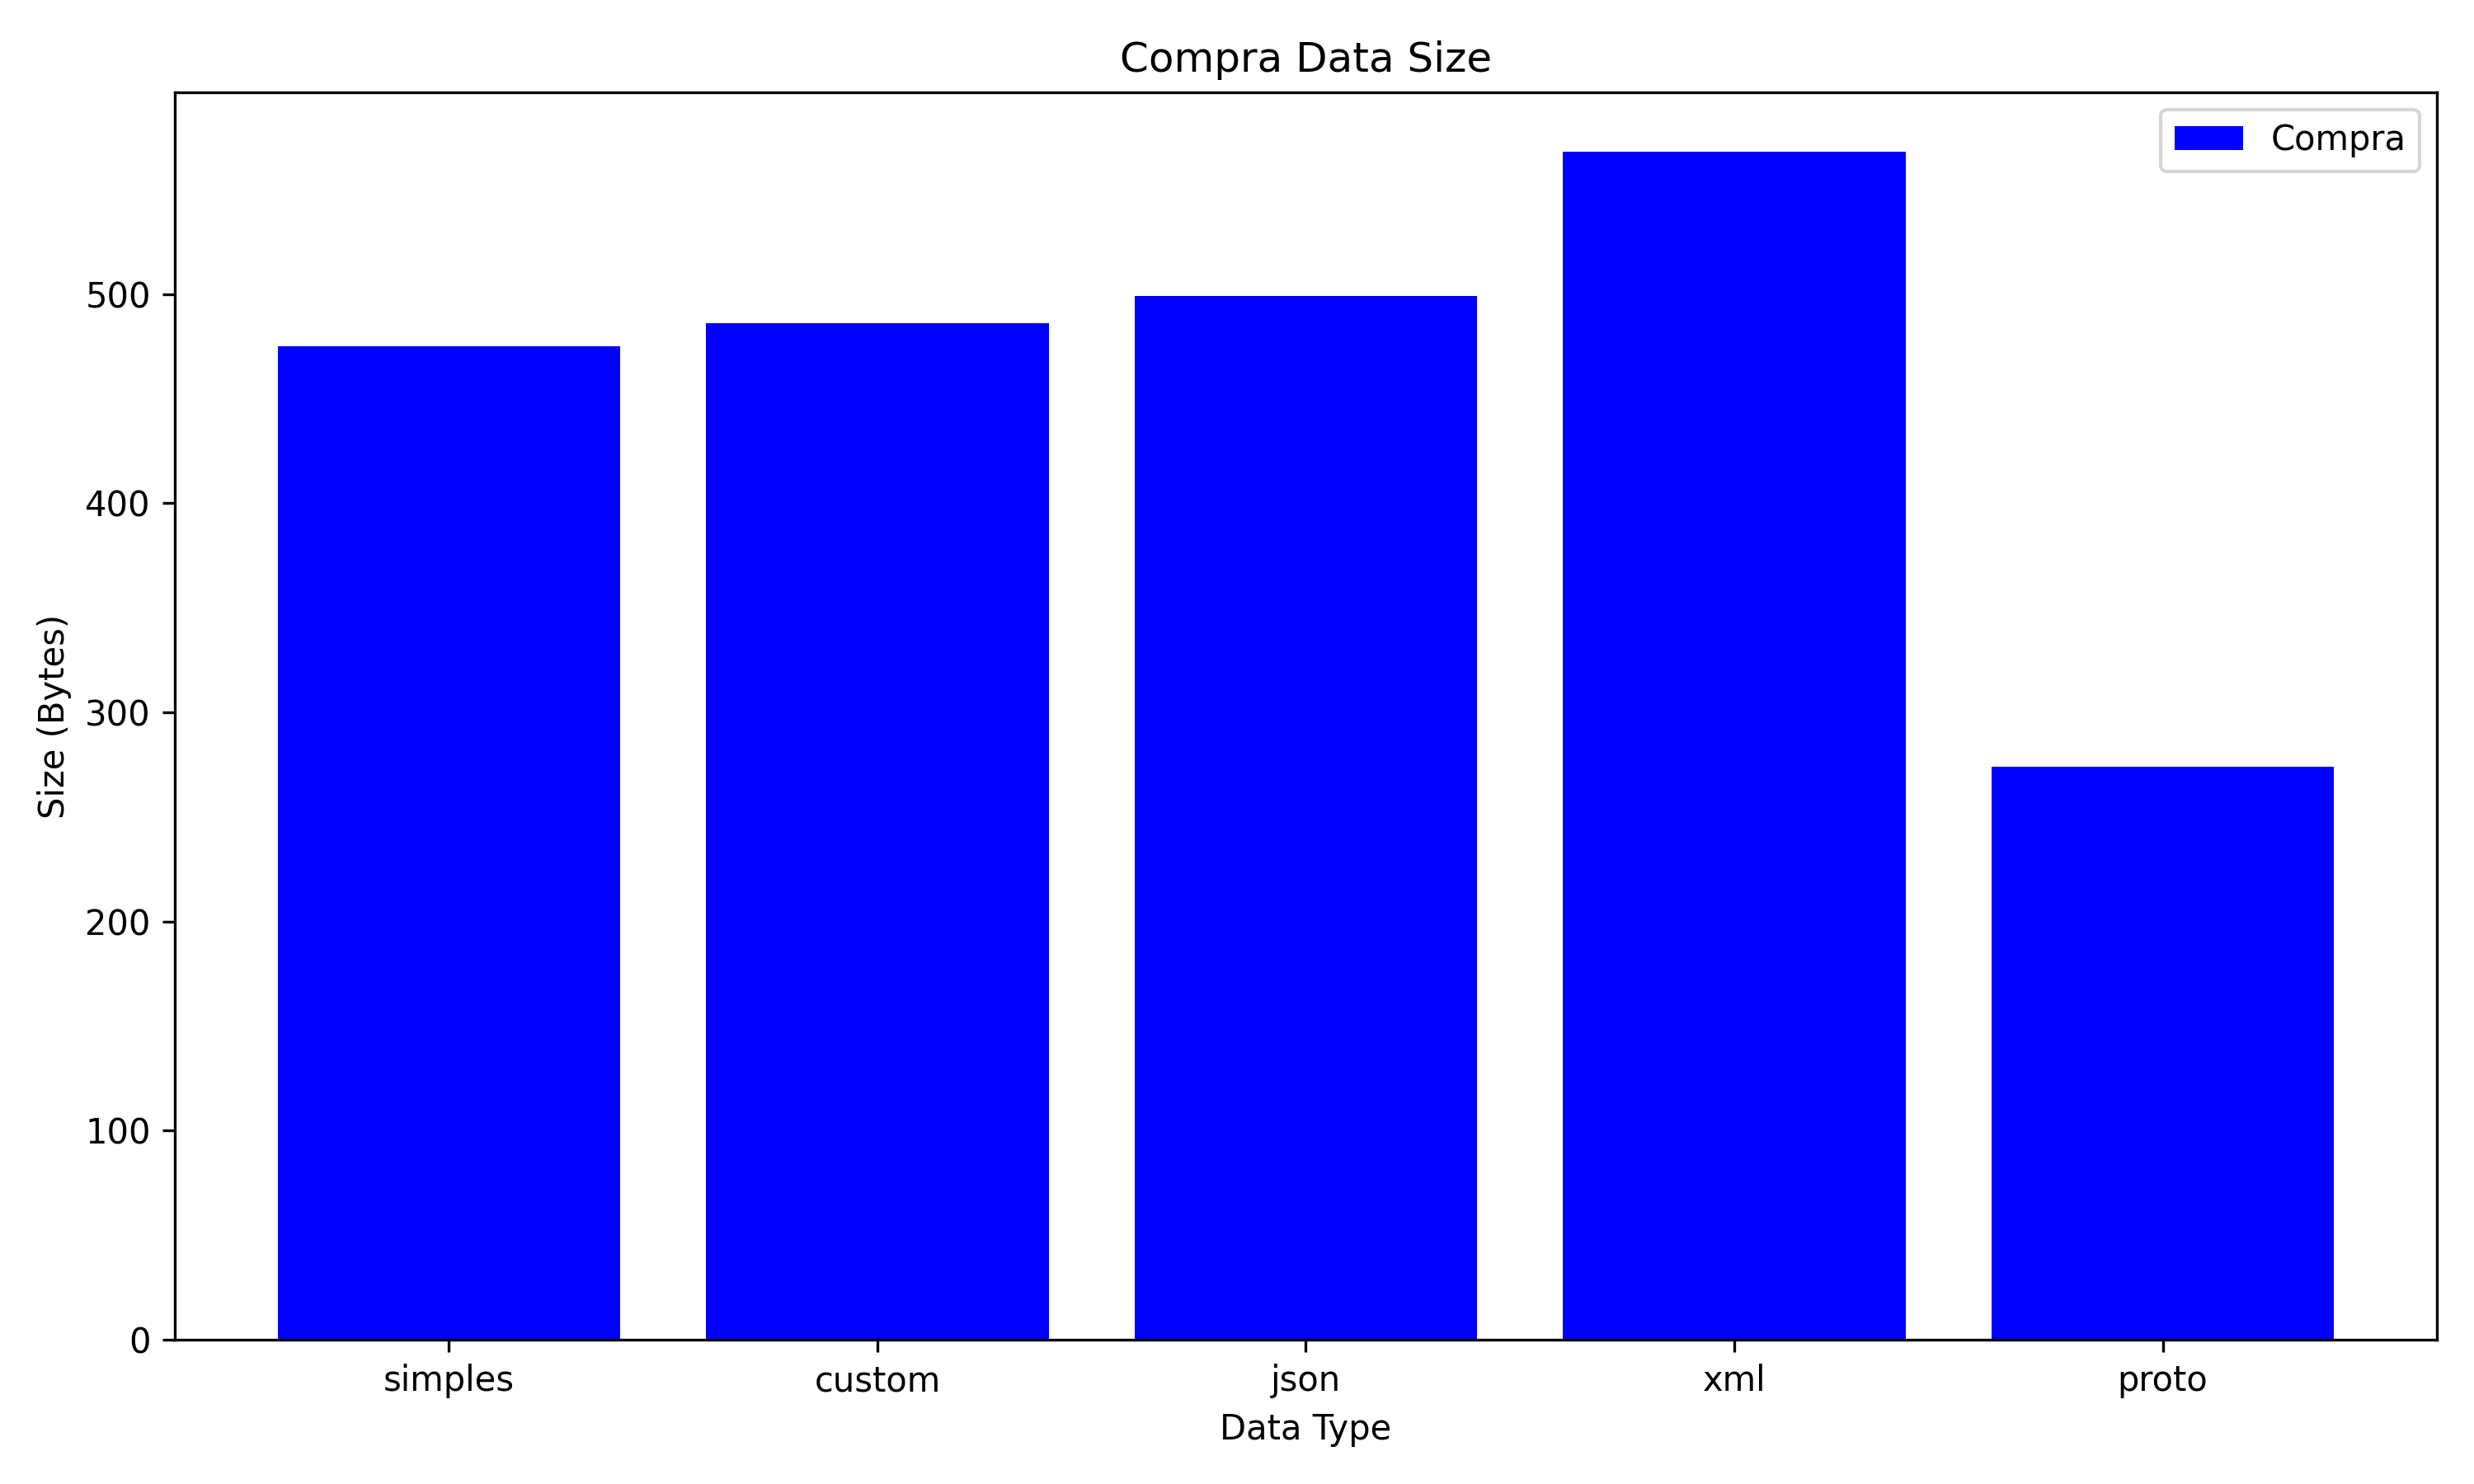
\includegraphics[width=\textwidth]{imgs/compra_data_size.png}
        \caption{Execução dos processos servidor e cliente com protocolo de serialização padrão do Java.}
        \label{fig:clock_original}
    \end{subfigure}%

    \begin{subfigure}[b]{0.7\textwidth}
        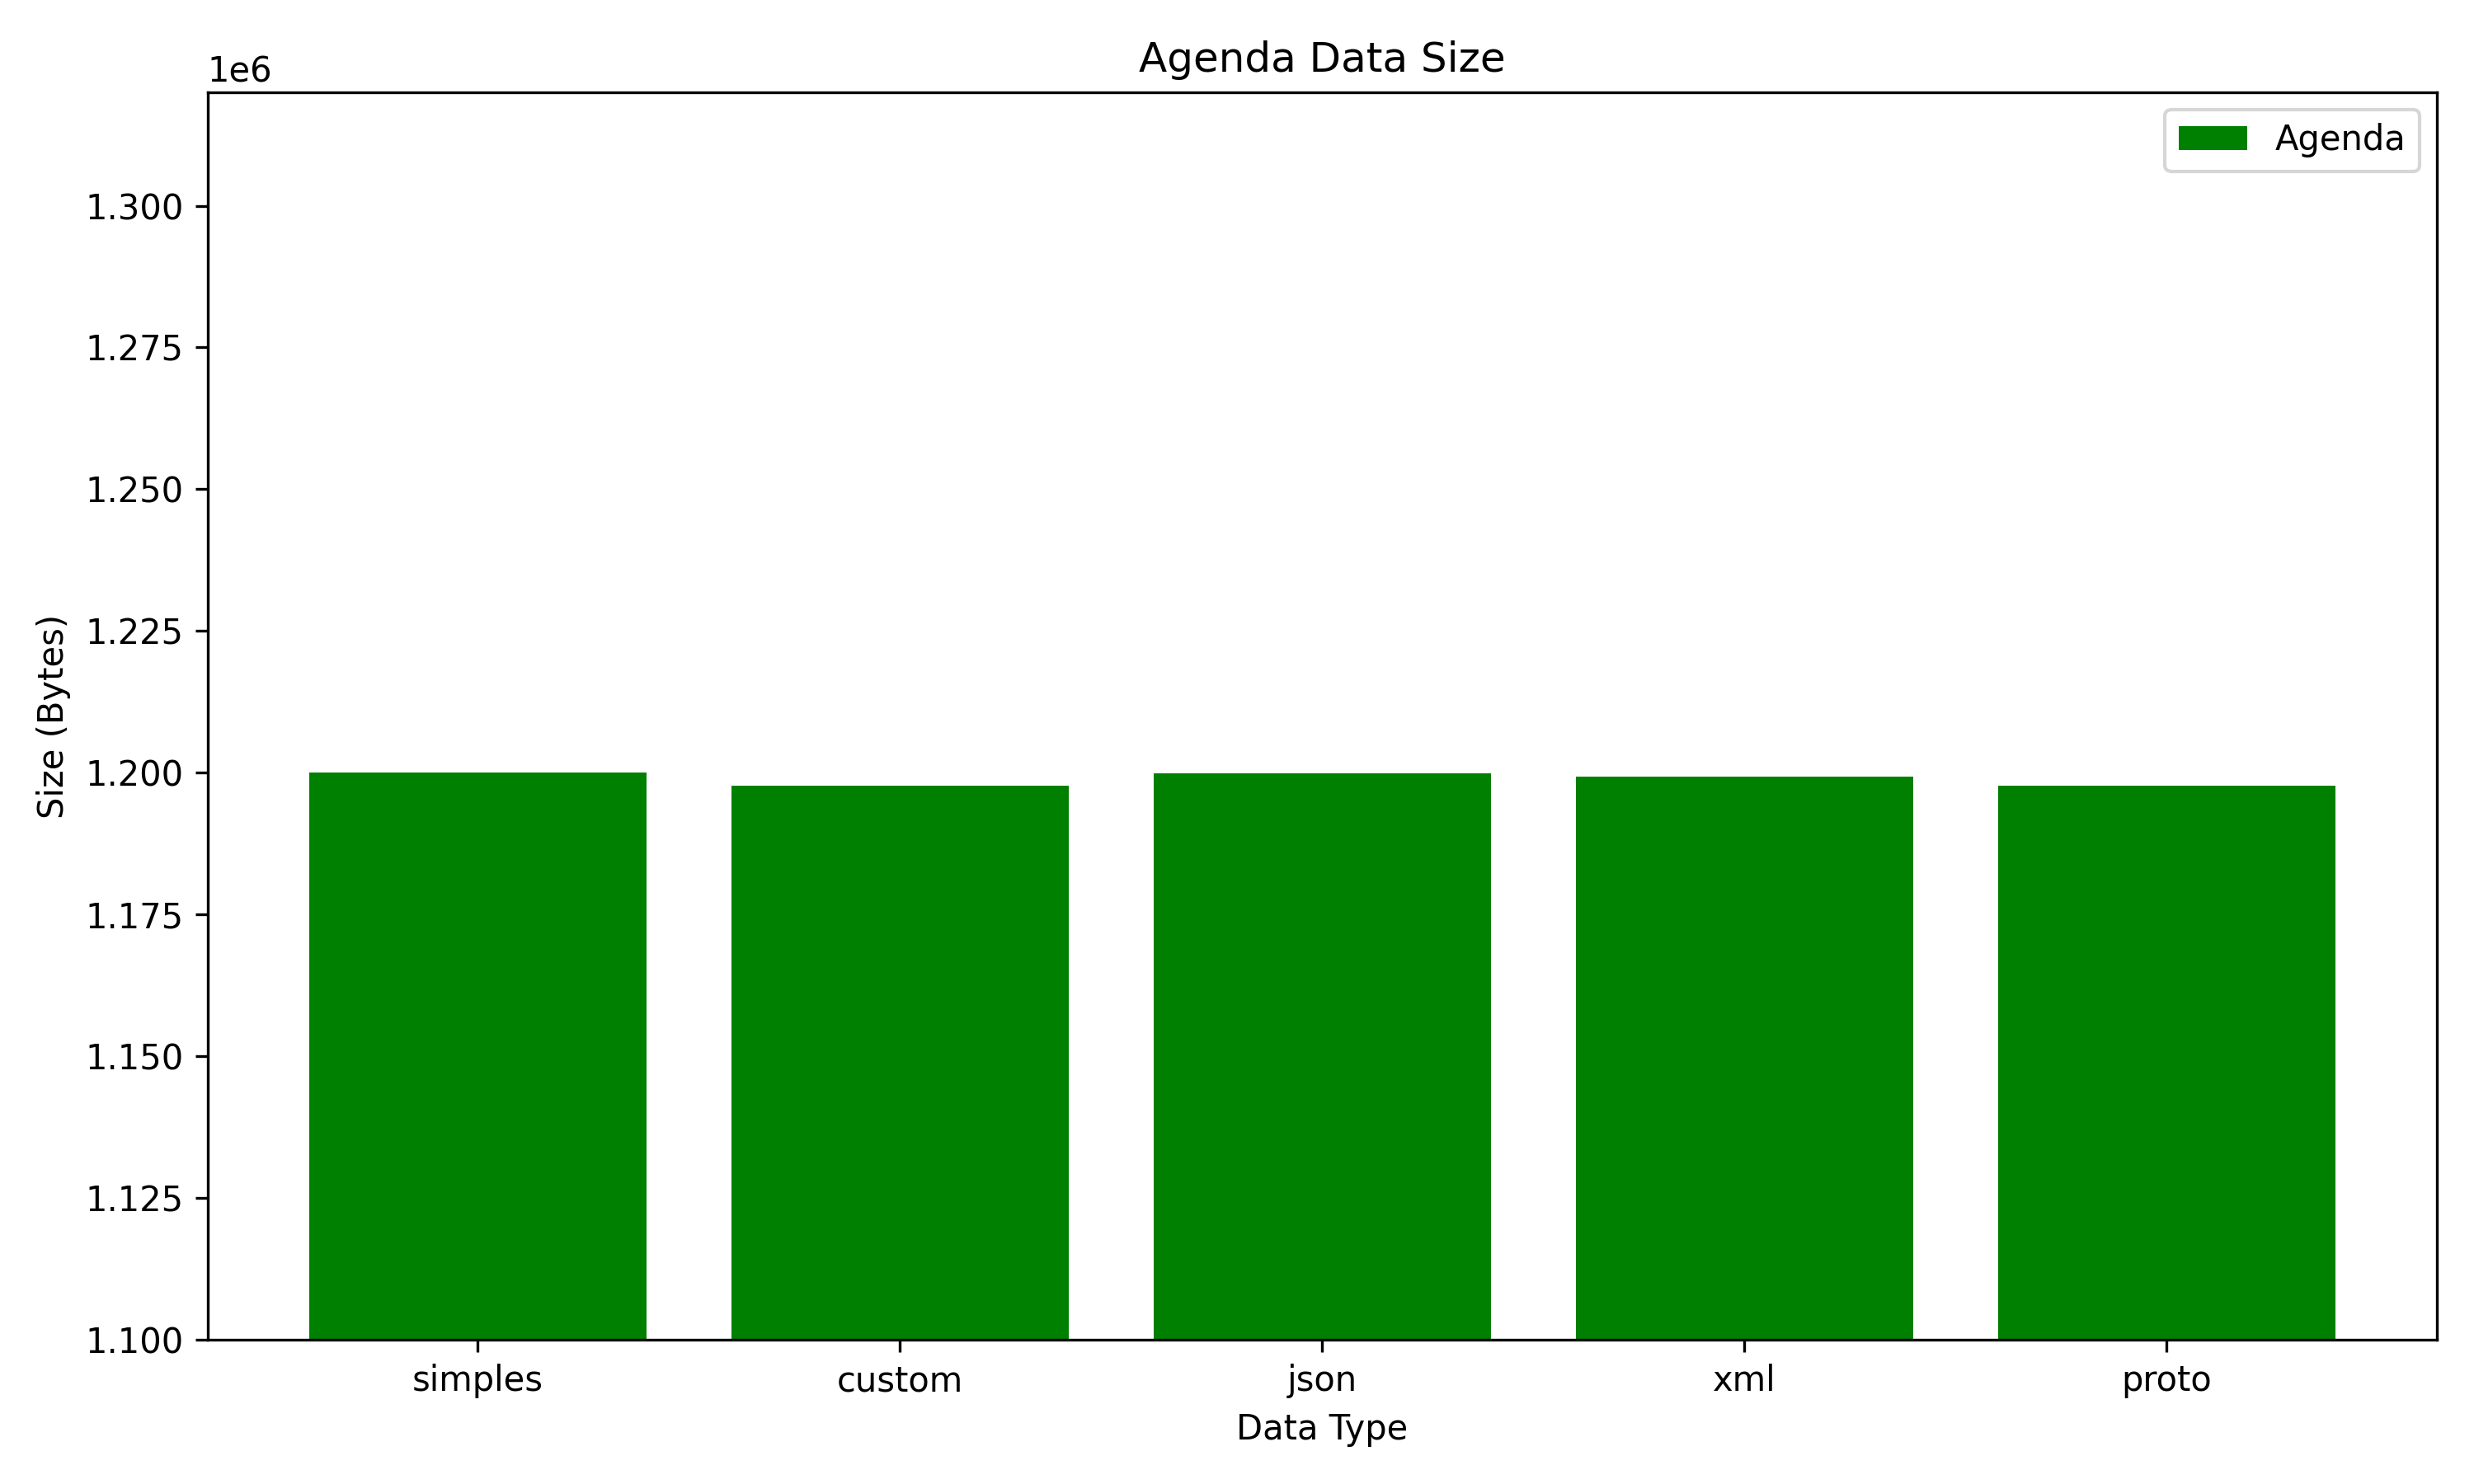
\includegraphics[width=\textwidth]{imgs/agenda_data_size.png}
        \caption{Captura dos pacotes trocados pelos processos cliente e servidor com protocolo de serialização padrão do Java.}
        \label{fig:clock_300dpi}
    \end{subfigure}%
    \label{fig:clock_comparison}
\end{figure}

Aplicamos o mesmo raciocínio a outras duas imagens escolhidas: imagem do coqueiro e imagem da chuva.

% \begin{figure}[H]
%     \centering
%     \caption{Imagens do coqueiro.}
%     \begin{subfigure}[b]{0.3\textwidth}
%         \includegraphics[width=\textwidth]{imgs/2.1.png}
%         \caption{Imagem original 300 dpi.}
%     \end{subfigure}%
%     \hfill
%     \begin{subfigure}[b]{0.3\textwidth}
%         \includegraphics[width=\textwidth]{imgs/2.2.png}
%         \caption{Imagem modificada com 60 dpi.}
%     \end{subfigure}%
%     \hfill
%     \begin{subfigure}[b]{0.3\textwidth}
%         \includegraphics[width=\textwidth]{imgs/2.3.png}
%         \caption{Imagem modificada com 300 dpi.}
%     \end{subfigure}
%     \hfill
%     \caption{Imagens diferença do coqueiro.}
%     \begin{subfigure}[b]{0.3\textwidth}
%         \includegraphics[width=\textwidth]{imgs/dif2.1.png}
%         \caption{Imagem de diferença da imagem original (300 dpi) com a de 60 dpi.}
%     \end{subfigure}%
%     \hfill
%     \begin{subfigure}[b]{0.3\textwidth}
%         \includegraphics[width=\textwidth]{imgs/dif2.2.png}
%         \caption{Imagem de diferença da imagem original (300 dpi) com a de 300 dpi interpolada.}
%     \end{subfigure}%
% \end{figure}

% \begin{figure}{H}
%     \centering
%     \caption{Imagens da chuva.}
%     \begin{subfigure}[b]{0.3\textwidth}
%         \includegraphics[width=\textwidth]{imgs/3.1.png}
%         \caption{Imagem original 300 dpi.}
%     \end{subfigure}%
%     \hfill
%     \begin{subfigure}[b]{0.3\textwidth}
%         \includegraphics[width=\textwidth]{imgs/3.2.png}
%         \caption{Imagem modificada com 60 dpi.}
%     \end{subfigure}%
%     \hfill
%     \begin{subfigure}[b]{0.3\textwidth}
%         \includegraphics[width=\textwidth]{imgs/3.3.png}
%         \caption{Imagem modificada com 300 dpi.}
%     \end{subfigure}
%     \hfill
%     \caption{Imagens diferença da chuva.}
%     \begin{subfigure}[b]{0.3\textwidth}
%         \includegraphics[width=\textwidth]{imgs/dif3.1.png}
%         \caption{Imagem de diferença da imagem original (300 dpi) com a de 60 dpi.}

%     \end{subfigure}%
%     \hfill
%     \begin{subfigure}[b]{0.3\textwidth}
%         \includegraphics[width=\textwidth]{imgs/dif3.2.png}
%         \caption{Imagem de diferença da imagem original (300 dpi) com a de 300 dpi interpolada.}
%     \end{subfigure}%
% \end{figure}
\vbox{} Conclui-se que, em determinadas condições, a interpolação bilinear é um ótimo método para interpolar pixels a uma imagem. Em especial, quando a diferença de intensidade entre pixels vizinhos é considerável, a interpolação é uma boa estratégia para aumentar a densidade de pixels (dpi). Além disso, por ser uma média ponderada, a interpolação bilinear acaba suavizando a diferença de intensidade entre pixels de uma imagem.
\section{Código Fonte em C++}
% \lstinputlisting[language=C++, caption={Código fonte do programa de interpolação bilinear em C++.}]{main.cpp}
% \lstinputlisting[language=C++, caption={Código fonte do programa de diferença de imagens em C++.}]{dif_tif.cpp}

\end{document}